\documentclass{article}

%% Denote paragraphs with vertical space rather than indenting (not critical)
\usepackage{parskip}

%% Support for URL in introductory text (not needed for main example)
\usepackage{url}

%% *** Enable TikZ ***
\usepackage{tikz}

%% *** TikZ library ***
\usetikzlibrary{arrows.meta,calc}

\begin{document}

%% Introductory Text
Example 2.18 from the book\\
\emph{Unlocking LaTeX Graphics: A Concise Guide to Ti$k$Z/PGF and PGFPLOTS}.\\
For more information, visit \url{https://latex-graphics.com}.
\par\bigskip

%% *** START OF EXAMPLE CODE ***
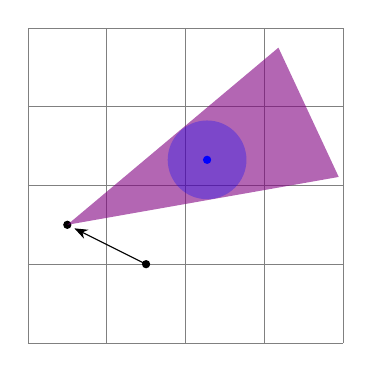
\begin{tikzpicture}[ >=Stealth,
    wedge/.style={violet,fill opacity=.60},
    bigcirc/.style={blue,fill opacity=0.3}]
  \draw[help lines] grid(4,4);
  \fill (0.5,1.5) coordinate (A) circle(1.5pt);
  \fill[wedge] ($(A)+(40:3.5)$) -- (A) --
    ($(A)+(10:3.5)$);
  \fill (1.5,1) coordinate (B) circle(1.5pt);
  \draw[->,shorten >=1mm] (B) -- (A);
  \coordinate (C) at (2.275,2.325);
  \fill[bigcirc] (C) circle(0.5cm);
  \fill[blue] (C) circle(1.5pt);
\end{tikzpicture}
%% *** END OF EXAMPLE CODE ***

\end{document}
